\documentclass{article}

\usepackage{lipsum}
\usepackage{amsfonts}
\usepackage{amsmath}
\usepackage{amsthm}
\usepackage{graphicx}
\graphicspath{{figures/4_21_22/}}
\usepackage{epstopdf}
\ifpdf%
\DeclareGraphicsExtensions{.eps,.pdf,.png,.jpg}
\else
\DeclareGraphicsExtensions{.eps}
\fi
\usepackage{amsopn}
\DeclareMathOperator{\diag}{diag}
\usepackage{booktabs}
\usepackage{bbm}
\usepackage{bm}
\usepackage{caption}
\usepackage{subcaption}
\usepackage[utf8]{inputenc}
\usepackage[T1]{fontenc}
\usepackage[margin=1in]{geometry}
\usepackage{hyperref}
\usepackage{algorithm}
\usepackage{algpseudocode}
\usepackage{placeins}

\newcommand{\norm}[1]{\left\lVert#1\right\rVert}
\newcommand{\normtwo}[1]{\left\lVert#1\right\rVert_2}
\newcommand{\abs}[1]{\left\lvert#1\right\rvert}
\newcommand{\mat}[1]{\bm{{#1}}}
\renewcommand{\vec}[1]{\bm{{#1}}}
\newcommand{\lequiv}{\Leftrightarrow}
\newcommand{\bigO}[1]{\mathcal{O}\!\left(#1\right)}
\newcommand{\ceil}[1]{\left\lceil #1 \right\rceil}
\newcommand{\floor}[1]{\left\lfloor #1 \right\rfloor}
\newcommand{\sfrac}[2]{#1/#2}
\newcommand{\hquad}{\enskip}
\newcommand{\expected}[1]{\mathbb{E}\left[#1\right]}
\newcommand{\mspan}[1]{\text{span}\left( #1 \right)}
\newcommand{\prob}[1]{P\left(#1\right)}
\newcommand{\probt}[1]{P\left( \text{#1} \right)}
\newcommand{\condprob}[2]{P\left(#1 \:|\: #2\right)}
\newcommand{\condprobt}[2]{P\left(\text{#1} \:|\: \text{#2}\right)}
\newcommand{\bayes}[2]{\frac{\condprob{#2}{#1}\prob{#1}}{\prob{#2}}}
\newcommand{\bayesx}[3]{\frac{\condprob{#2}{#1}\prob{#1}}{\condprob{#2}{#1}\prob{#1} + \condprob{#2}{#3}\prob{#3}}}
\newcommand{\sech}{\text{sech}}
\newcommand*{\vertbar}{\rule[-1ex]{0.5pt}{2.5ex}}
\newcommand*{\horzbar}{\rule[.5ex]{2.5ex}{0.5pt}}
\newcommand{\vect}[2]{\underline{{#1}}_{{#2}}}
\newcommand{\basisp}[1]{\underline{{p}}_{{#1}}}
\newcommand{\basisq}[1]{\underline{{q}}_{{#1}}}
\newcommand{\coeff}[1]{\underline{{a}}_{{#1}}}
\newcommand{\bestfit}{\underline{\bar{x}}}
\newcommand{\grad}{\nabla}
\newcommand{\laplace}{\Delta}
\newcommand{\setbar}{\:\middle|\:}
\renewcommand{\div}{\grad \cdot}
\renewcommand{\Re}{\text{Re}}
\newcommand{\var}[1]{\texttt{{#1}}}

\begin{document}
\section{Background}
Learning aggregation for 3D anisotropic diffusion on a structured grid
\begin{equation}
  -\grad \cdot \left(\mat{D} \grad u\right) = 0,
\end{equation}
\begin{equation}
  %\mat{D} = \begin{bmatrix} \cos \theta & -\sin \theta \\ \sin \theta & \cos \theta \end{bmatrix} \begin{bmatrix} 1 & \\ & \varepsilon \end{bmatrix} \begin{bmatrix} \cos \theta & -\sin \theta \\ \sin \theta & \cos \theta \end{bmatrix}^T,
  \mat{D} := \mat{R}^T\begin{bmatrix}\varepsilon_x & & \\ & \varepsilon_y & \\ & & 1 \end{bmatrix}\mat{R},
\end{equation}
\begin{equation}
  \mat{R} := \begin{bmatrix} \cos \theta_z & -\sin \theta_z & 0 \\ \sin \theta_z & \cos \theta_z & 0 \\ 0 & 0 & 1\end{bmatrix} \begin{bmatrix}\cos \theta_y & 0 & \sin \theta_y \\ 0 & 1 & 0 \\ -\sin\theta_y & 0 & \cos\theta_y \end{bmatrix}.
\end{equation}
For now, this is on the specific problem for $N_x=N_y=N_z=12$ (number of elements in each dimension), $\theta_z=1.11\pi$, $\theta_y=0.58\pi$, $\varepsilon_x=0.001$, $\varepsilon_y=1000.0$.

This was discretized in Firedrake \cite{Firedrake} using piecewise linear tetrahedral finite elements with homogeneous Dirichlet boundary conditions.  Afterwards, the degrees-of-freedom corresponding to the Dirichlet boundary were removed from the system.  Overall, there are $11 \times 11 \times 11 = 1331$ degrees of freedom total.

\begin{figure}[h]
  \centering
  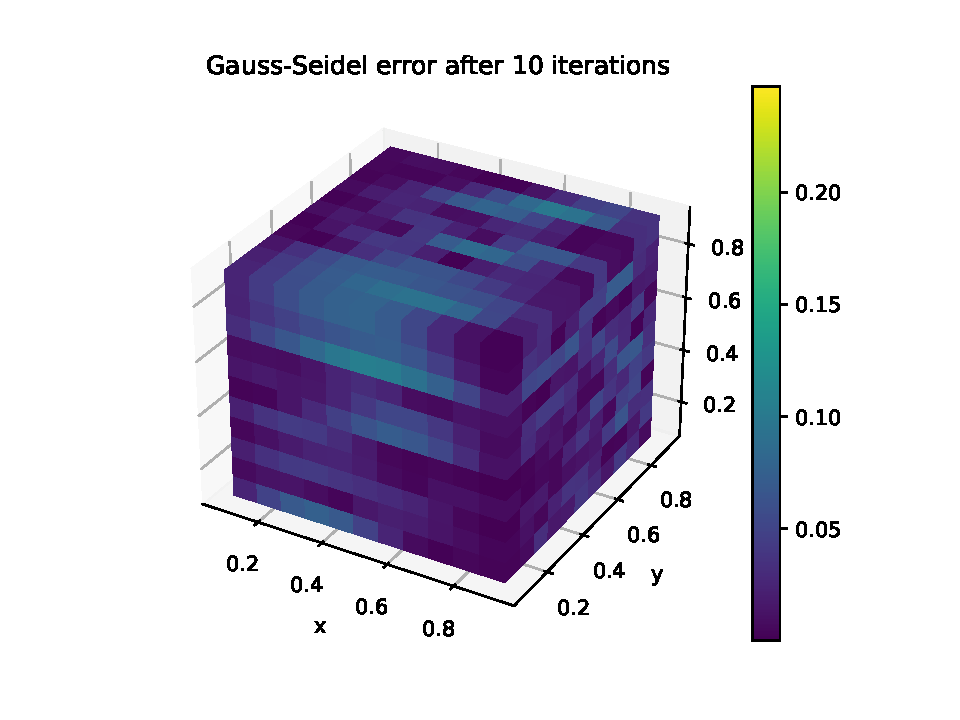
\includegraphics[width=0.8\textwidth]{gs_error.pdf}
  \caption{Error behavior on the problem with a random initial guess, solving $\mat{Ax}=\mat{0}$ with Gauss-Seidel iterations.  The direction and strength of anisotropy are visible by looking at in which areas the error is geometrically smooth.}
  \label{fig:gs_error}
\end{figure}

\begin{figure}[h!]
  \centering
  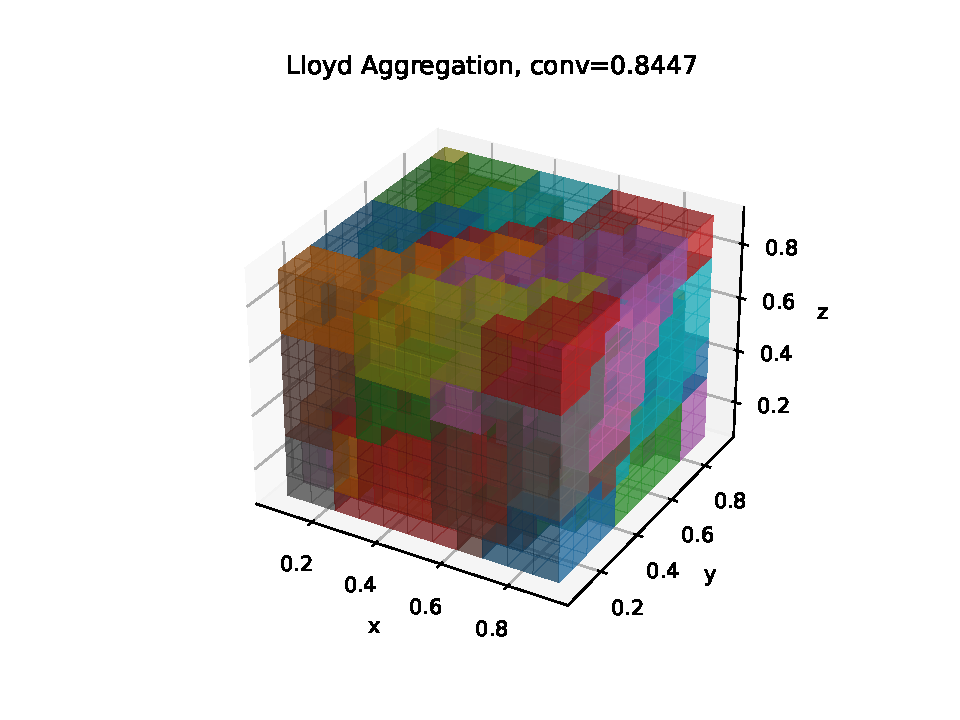
\includegraphics[width=0.8\textwidth]{lloyd_agg.pdf}
  \caption{Aggregate selection when using PyAMG's (regular) Lloyd aggregation \cite{OlSc2018}.}
  \label{fig:lloyd_agg}
\end{figure}

\begin{figure}[h!]
  \centering
  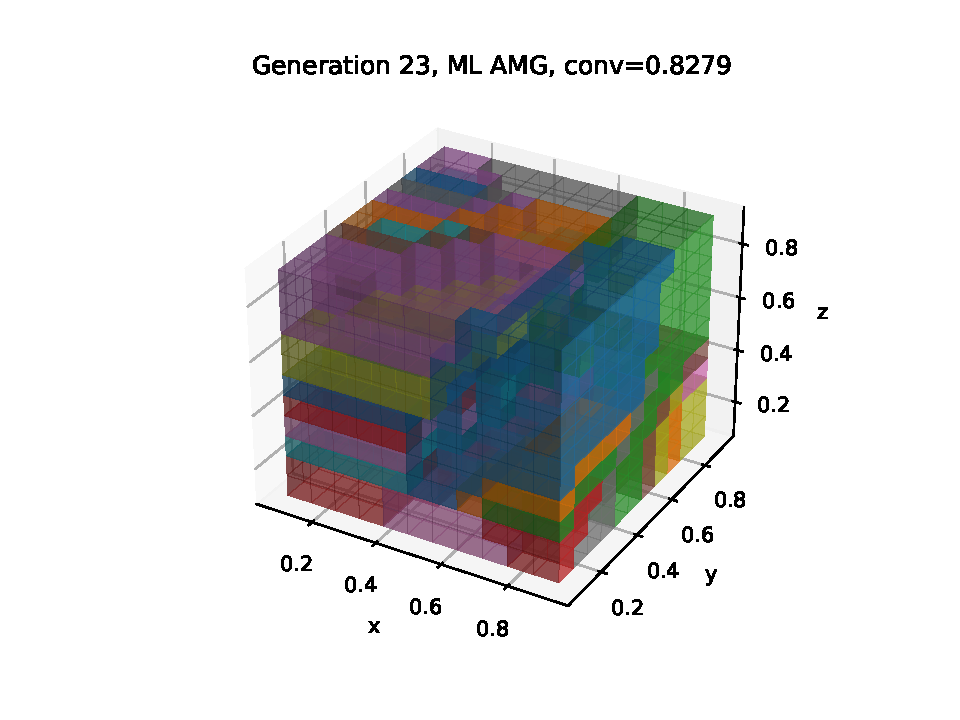
\includegraphics[width=0.8\textwidth]{ml_agg.pdf}
  \caption{Aggregate selection from the ML method.  This is trained on the specific problem being shown.}
  \label{fig:ml_agg}
\end{figure}

\bibliographystyle{siam}
\bibliography{navier}
\end{document}
